\begin{SCn}
	
\scnsectionheader{\currentname}
	
\scnstartsubstruct
	
\scnheader{Предметная область искусственных нейронных сетей}
\scnidtf{Предметная область и.н.с.}
\scniselement{предметная область}
\scnsdmainclass{искусственная нейронная сеть;действие с искусственной нейронной сетью}
\scnsdclass{
    искусственная нейронная сеть;
    искусственная нейронная сеть с прямыми связями;
    персептрон;
    персептрон Розенблатта;
    персептрон Румельхарта;
    автоэнкодерная искусственная нейронная сеть;
    машина опорных векторов;
    искусственная нейронная сеть радиально-базисных функций;
    искусственная нейронная сеть с обратными связями;
    рекуррентная искусственная нейронная сеть;
    искусственная нейронная сеть Джордана;
    искусственная нейронная сеть Элмана;
    LSTM-элемент;
    GRU-элемент;
    полносвязная искусственная нейронная сеть;
    слабосвязная искусственная нейронная сеть;
    нейрон;
    полносвязный нейрон;
    сверточный нейрон;
    рекуррентный нейрон;
    синапс;
    параметр нейронной сети;
    параметр обучения нейронной сети;
    целевой параметр обучения нейронной сети;
    весовой коэффициент;
    ядро свертки;
    параметр архитектуры нейронной сети;
    количество слоев;
    количество нейронов;
    количество синапсов;
    образ;
    признак;
    слой;
    полносвязный слой;
    сверточный слой;
    слой нелинейного преобразования;
    dropout слой;
    pooling слой;
    действие обработки и.н.с.
}
\scnsdrelation{
    нейрон';
    пороговый нейрон';
    синапс';
    входное значение*;
    выходное значение*;
    функция активации*;
    взвешенная сумма*;
    распределяющий слой*;
    обрабатывающий слой*;
    выходной слой*
}

\scnrelfrom{частная предметная область}{
Предметная область обучения искусственных нейронных сетей
}


%\scnrelfromset{частная предметная область}{
%Предметная область ИНС с заданным направлением связей\\
%    \scnaddlevel{1}
%    \scnrelfromset{частная предметная область}{
%    Предметная область ИНС с прямым связями\\
%        \scnaddlevel{1}
%        \scnrelfromset{частная предметная область}{
%        Предметная область персептронов\\
%            \scnaddlevel{1}
%            \scnrelfromset{частная предметная область}{
%            Предметная область персептронов Розенблатта
%            ;Предметная область персептронов Румельхарта
%            ;Предметная область автоэнкодерных ИНС
%            }
%            \scnaddlevel{-1}
%        ;Предметная область ИНС радиально-базисных функций
%        ;Предметная область машин опорных векторов
%        }
%        \scnaddlevel{-1}
%    ;Предметная область ИНС с обратными связями\\
%        \scnaddlevel{1}
%        \scnidtf{Предметная область рекуррентных ИНС}
%        \scnrelfromset{частная предметная область}{
%        Предметная область ИНС Джордана
%        ;Предметная область ИНС Элмана
%        ;Предметная область LSTM-элементов
%        ;Предметная область GRU-элементов
%        }
%        \scnaddlevel{-1}
%    }
%    \scnaddlevel{-1}
%;Предметная область обучения ИНС\\
%    \scnaddlevel{1}
%    \scnrelfromset{частная предметная область}{
%    Предметная область ИНС, обучающихся с учителем
%    ;Предметная область ИНС, обучающихся без учителя\\
%        \scnaddlevel{1}
%        \scnrelfromset{частная предметная область}{
%        Предметная область обучающихся автоэнкодерных ИНС
%        ;Предметная область ИНС глубокого доверия
%        ;Предметная область генеративно-состязательных ИНС
%        ;Предметная область самоорганизующихся карт Кохонена
%        ;Предметная область ИНС Хопфилда
%        ;Предметная область подкрепляющего обучения ИНС
%        }
%        \scnaddlevel{-1}
%    }
%    \scnaddlevel{-1}
%;Предметная область топологий ИНC\\
%    \scnaddlevel{1}
%    \scnrelfromset{частная предметная область}{
%    Предметная область полносвязных ИНC
%    ;Предметная область многослойных ИНC
%    ;Предметная область слабосвязных ИНC
%    }
%    \scnaddlevel{-1}
%;Предметная область задач, решаемых с помощью ИНС\\
%    \scnaddlevel{1}
%    \scnrelfromset{частная предметная область}{
%    Предметная область ИНС, решающих задачу классификации
%    ;Предметная область ИНС, решающих задачу аппроксимации
%    ;Предметная область ИНС, решающих задачу управления
%    ;Предметная область ИНС, решающих задачу фильтрации
%    ;Предметная область ИНС, решающих задачу детекции
%    ;Предметная область ИНС, решающих задачу с ассоциативной памятью
%    }
%    \scnaddlevel{-1}
%;Предметная область интеграции ИНС с базой знаний
%}

\scnheader{искусственная нейронная сеть}
    \scnidtf{и.н.с.}
    \scnidtf{множество искусственных нейронных сетей}
    \scnidtf{нейронная сеть}
    \scndefinition{
        \textbf{\textit{искусственная нейронная сеть}} -- это совокупность нейронных элементов и связей между ними (\scncite{Golovko2017}).

        Искусственная нейронная сеть состоит из \textbf{\textit{нейронов}}. Нейроны связанны между собой посредством
        \textbf{\textit{синапсов}}. Нейроны организованы в \textbf{\textit{слои}}. Каждый нейрон слоя принимает сигналы
        со входящих в него синапсов, обрабатывает их единым образом с помощью заданной ему или всему слою
        \textbf{\textit{функции активации}} и передает результат на выходящие из него синапсы.
    }
    \scnexplanation{
        \textbf{\textit{Искусственная нейронная сеть}} - это биологически инспирированная математическая модель,
        обладающая обобщающей способностью после выполнения процедуры обучения. Под обобщающей способностью понимается способность
        модели выдавать корректные результаты для экземпляров, не входящих в обучающую выборку.
    }
    \scnsubset{математическая модель}
    \scnaddlevel{1}
        \scnexplanation{\textbf{\textit{математическая модель}} - это упрощенное описание объекта реального мира, выраженное с помощью математической символики}
    \scnaddlevel{-1}

    \scnrelfrom{изображение}{
        \scnfileimage{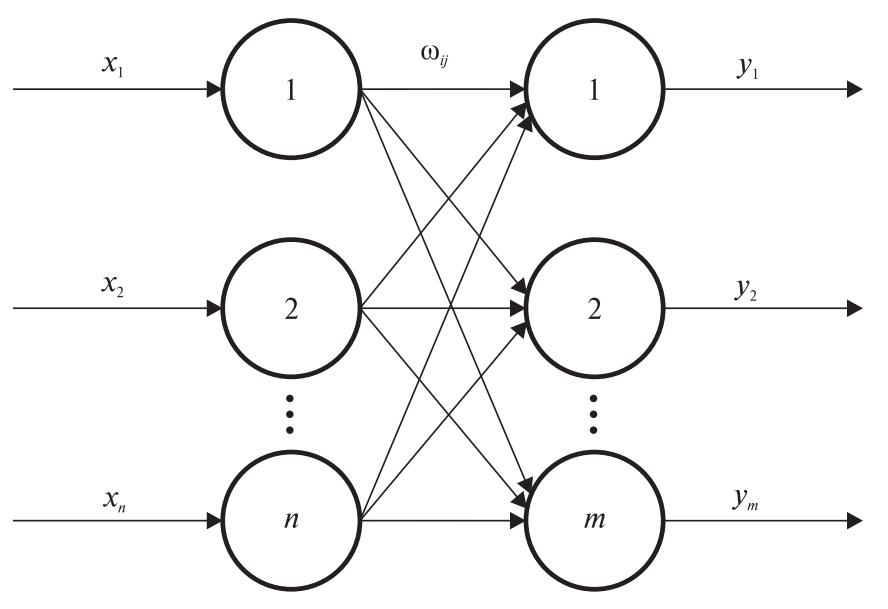
\includegraphics[width=0.4\linewidth]{figures/sd_ps/sd_ann/neural_network.png}}
    }

    \scnrelfrom{описание типичного экземпляра}{
        \scnfilescg{figures/sd_ps/sd_ann/neural_network_scg.png}
    }

    \scnrelfrom{разбиение}{\scnkeyword{Типология и.н.с. по признаку направленности связей\scnsupergroupsign}}
    \scnaddlevel{1}
        \scneqtoset{
        искусственная нейронная сеть с прямыми связями\\
        \scnaddlevel{1}
            \scnsubdividing{
                персептрон\\
                \scnaddlevel{1}
                    \scnsubdividing{
                        персептрон Розенблатта;
                        персептрон Румельхарта;
                        автоэнкодерная искусственная нейронная сеть
                    }
                \scnaddlevel{-1}
                ;машина опорных векторов
                ;искусственная нейронная сеть радиально-базисных функций
            }
        \scnaddlevel{-1}
        ;искусственная нейронная сеть с обратными связями
        \scnaddlevel{1}
            \scnidtf{рекуррентная искусственная нейронная сеть}
            \scnsubdividing{
            искусственная нейронная сеть Джордана
            ;искусственная нейронная сеть Элмана
            ;LSTM-элемент
            ;GRU-элемент
            }
        \scnaddlevel{-1}
        }
    \scnaddlevel{-1}

    \scnrelfrom{разбиение}{\scnkeyword{Типология и.н.с. по признаку полноты связей\scnsupergroupsign}}
    \scnaddlevel{1}
        \scneqtoset{
        полносвязная искусственная нейронная сеть\\
        ;слабосвязная искусственная нейронная сеть
        }
    \scnaddlevel{-1}

    \scnrelfrom{решаемые задачи}{задачи, которые могут быть решены с помощью и.н.с. с приемлемой точностью}{
    \scnaddlevel{1}
    \scneqtoset{
        задача классификации\\
        \scnaddlevel{1}
            \scnsubset{задача}
            \scnexplanation{задача построения классификатора, т.е. отображения $\tilde c: X \rightarrow C$, где $ X \in \mathbb{R}^m$ --
            признаковое пространство экземпляров, $C = {C_1, C_2, ...C_k }$ -- конечное и обычно небольшое множество меток классов.}
        \scnaddlevel{-1}
        ;задача регрессии\\
        \scnaddlevel{1}
            \scnsubset{задача}
            \scnexplanation{задача построения оценочной функции по примерам $(x_i, f(x_i))$, где $f(x)$ -- неизвестная функция}
        \scnaddlevel{-1}
        ;задача кластеризация\\
        \scnaddlevel{1}
            \scnsubset{задача}
            \scnexplanation{задача разбиения множества экземпляров на группы (кластеры) по какой-либо метрике сходства}
        \scnaddlevel{-1}
        ;задача понижения размерности\\
        \scnaddlevel{1}
            \scnsubset{задача}
            \scnidtf{задача уменьшения размерности признакового пространства}
        \scnaddlevel{-1}
        ;задача управления\\
        \scnaddlevel{1}
            \scnsubset{задача}
        \scnaddlevel{-1}
        ;задача фильтрации\\
        \scnaddlevel{1}
            \scnsubset{задача}
        \scnaddlevel{-1}
        ;задача детекции\\
        \scnaddlevel{1}
            \scnsubset{задача}
            \scnsubset{задача классификации}
            \scnsubset{задача регрессии}
        \scnaddlevel{-1}
        ;задача с ассоциативной памятью\\
        \scnaddlevel{1}
            \scnsubset{задача}
        \scnaddlevel{-1}
    }
    }

\scnheader{нейрон}
    \scnidtf{искусственный нейрон}
    \scnidtf{формальный нейрон}
    \scnidtf{нейронный элемент}
    \scnidtf{множество нейронов искусственных нейронных сетей}
    \scnidtf{математическая модель реального биологического нейрона}
    \scnnote{отдельный нейрон является искусственной нейронной сети с одним нейроном в единственном слое}
    \scnsubset{искусственная нейронная сеть}
    \scndefinition{
        \textbf{\textit{нейрон}} – это основной элемент \textit{искусственной нейронной сети}, применяющий свою \textit{функцию активации} к
            сумме произведений входных сигналов на весовые коэффициенты (\scncite{Golovko2017}):
        \begin{equation*}
            y = F\left(\sum_{i=1}^{n} w_ix_i\right) = F(WX)
        \end{equation*}
        где $X = (x_1,x_2,...,x_n)^{T}$ – вектор входного сигнала; $W - (w_1,w_2,...,w_n)$ - вектор весовых коэфициентов;
        \textit{F} -- функция активации.
    }

    \scnrelfrom{изображение}{
        \scnfileimage{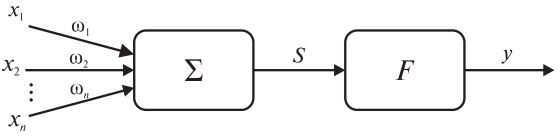
\includegraphics[width=0.4\linewidth]{figures/sd_ps/sd_ann/neuron.png}}
    }

    \scnnote{Нейроны могут иметь полный набор связей с нейронами предшествующего слоя или неполный (разряженный)
        набор связей.}

    \scnsubdividing{
        полносвязный нейрон\\
        \scnaddlevel{1}
            \scnidtf{нейрон, у которого есть полный набор связей с нейронами предшествующего слоя}
            \scnexplanation{отдельный обрабатывающий элемент и.н.с., выполняющий функциональное преобразование взвешенной суммы элементов вектора входных значений с помощью функции активации}
        \scnaddlevel{-1}
        ;сверточный нейрон\\
        \scnaddlevel{1}
            \scnexplanation{отдельный обрабатывающий элемент и.н.с., выполняющий функциональное преобразование результата
                операции свертки матрицы входных значений с помощью функции активации}
            \scnnote{Сверточный нейрон с соответствующим ему ядром свертки может быть представлен нейроном
                с неполным набором связей}
        \scnaddlevel{-1}
        ;рекуррентный нейрон\\
        \scnaddlevel{1}
            \scnexplanation{нейрон, имеющий обратную связь с самим собой или с другими нейронами и.н.с.}
        \scnaddlevel{-1}
    }

\scnheader{нейрон'}
    \scnidtf{нейронный элемент'}
    \scniselement{ролевое отношение}
    \scnrelfrom{первый домен}{искусственная нейронная сеть}
    \scnrelfrom{второй домен}{нейрон}
    \scnrelfrom{область определения}{искусственная нейронная сеть}
    \scndefinition{
        \textbf{\textit{нейрон'}} -- ролевое отношение, связывающее искусственную нейронную сеть с ее нейроном.
    }

\scnheader{пороговый нейрон'}
    \scnidtf{пороговый нейронный элемент'}
    \scniselement{ролевое отношение}
    \scnrelfrom{первый домен}{искусственная нейронная сеть}
    \scnrelfrom{второй домен}{нейрон}
    \scnrelfrom{область определения}{искусственная нейронная сеть}
    \scndefinition{
        \textbf{\textit{нейрон'}} -- ролевое отношение, связывающее искусственную нейронную сеть с таким ее нейроном,
            выходное значение которого всегда равно -1.
    }
    \scnexplanation{весовой коэффициент синапса, выходящего из такого нейрона, является порогом для нейрона, в который
        данный синапс входит}

\scnheader{синапс}
    \scnidtf{синаптическая связь}
    \scnsubset{ориентированная пара}
    \scndefinition{
        \textbf{\textit{синапс}} -- ориентированная пара, первым компонентом которой является нейрон, из которого исходит сигнал, а вторым компонентом -- нейрон, который принимает этот сигнал.
    }

\scnheader{синапс'}
    \scnidtf{синаптическая связь'}
    \scniselement{ролевое отношение}
    \scnrelfrom{первый домен}{искусственная нейронная сеть}
    \scnrelfrom{второй домен}{синапс}
    \scnrelfrom{область определения}{
        ...\\
        \scnreltoset{объединение}{искусственная нейронная сеть;синапс}
    }
    \scndefinition{
        \textbf{\textit{синапс'}} -- ролевое отношение, связывающее искусственную нейронную сеть с его синапсом.
    }

\scnheader{параметр нейронной сети}
    \scnsubset{параметр}
    \scnsubdividing{
        параметр обучения нейронной сети;
        целевой параметр обучения нейронной сети
        \scnaddlevel{1}
            \scnidtf{параметры, значения которых изменяются в ходе процесса обучения}
            \scnsubdividing{
                весовой коэффициент;
                ядро свертки
                \scnaddlevel{1}
                    \scnidtf{квадратная матрица произвольного порядка, элементы которой изменяются в процессе
                        обучения и.н.с.}
                \scnaddlevel{-1}
            }
        \scnaddlevel{-1}\\
        ;параметр архитектуры нейронной сети\\
        \scnaddlevel{1}
            \scnnote{набор параметров и.н.с., определяющих ее архитектуру}
            \scnsubdividing{количество слоев;количество нейронов; количество синапсов}
        \scnaddlevel{-1}
    }

\scnheader{весовой коэффициент}
    \scnidtf{вес синапса}
    \scnidtf{сила синаптической связи}
    \scnsubset{целевой параметр обучения нейронной сети}
    \scnexplanation{
        \textbf{\textit{весовой коэффициент}} - это числовой коэффициент, который ставится в соответствие каждому
        синапсу нейронной сети и изменяется в процессе обучения.
    }
    \scnnote{
        Если сила синаптической связи отрицательнена, то она называется \textit{тормозящей}. В противном случае она
        является \textit{усиливающей}.
    }

\scnheader{входное значение*}
    \scnidtf{входное значение нейрона*}
    \scniselement{неролевое отношение}
    \scniselement{бинарное отношение}
    \scnrelfrom{первый домен}{нейрон}
    \scnrelfrom{второй домен}{число}
    \scnrelfrom{область определения}{
        ...\\
        \scnreltoset{объединение}{нейрон;число}
    }
    \scndefinition{
        \textbf{\textit{входное значение*}} -- неролевое отношение, связывающее нейрон входного слоя с предобработанным
        значением признака образа, который подается на вход нейронной сети.
    }
    \scnexplanation{
        Предварительная обработка как правило включает в себя трансформацию категориальных признаков
        в численные, а также нормализацию, проектирование признаков и т.д.
    }
    \scntext{теоретическая неточность}{
        Использование множества как формы представления входных данных является серьезным допущением, так как на практике
        входные данные структурированы более сложно -- в многомерные массивы. Самым близким теоретическим аналогом
        здесь выступает тензор. К сожалению, описание теории нейроных сетей с помощью тензорного исчисления в литературе
        как таковое отсутствует, но активно используется на практике: например, во многих разрабатываемых нейросетевых фреймворках.
        Формализация нейронных сетей с помощью тензоров видится авторам наиболее вероятным направлением работы в
        ближайших изданиях стандарта OSTIS.
    }

\scnheader{образ}
    \scnidtf{instance}
    \scnidtf{экземпляр}
    \scniselement{мультимножество}
    \scniselement{ориентированное множество}
    \scndefinition{
        \textbf{\textit{образ}} -- ориентированное мультимножество численных и/или категориальных значений признаков некоторого объекта,
        которые могут выступать в качестве входных значений нейронов.
    }

\scnheader{признак}
    \scnidtf{feature}
    \scnidtf{множество признаков}
    \scnsubset{ролевое отношение}
    \scnexplanation{
        \textbf{\textit{признак}} - множество ролевых отношений, каждое из которых связывает некоторый образ с численным
        или категориальным значением, которое характеризует данный образ с какой-либо стороны.
    }

\scnheader{функция активации*}
    \scnidtf{функция активации нейрона*}
    \scniselement{неролевое отношение}
    \scniselement{бинарное отношение}
    \scndefinition{
        \textbf{\textit{функция активации*}} -- неролевое отношение, связывающее нейрон с функцией, результат
        применения которой к \textbf{\textit{взвешенной сумме нейрона}} определяет его \textbf{\textit{выходное значение}}.
    }
    \scnrelfrom{область определения}{
        ...\\
        \scnreltoset{объединение}{нейрон;функция}
    }
    \scnrelfrom{первый домен}{нейрон}
    \scnrelfrom{второй домен}{функция}
    \scnaddlevel{1}
    \scnsubdividing{
        линейная\\
        \scnaddlevel{1}
            \scnrelfrom{формула}{
                \begin{equation*}
                    y = kS
                \end{equation*}
                где \textit{k} -- коэффициент наклона прямой, \textit{S} -- в.с.
            }
        \scnaddlevel{-1}
        ;пороговая\\
        \scnaddlevel{1}
            \scnrelfrom{формула}{
                \begin{equation*}
                    y = sign(S) =
                    \begin{cases}
                        1, S > 0,\\
                        0, S \leq 0
                    \end{cases}
                \end{equation*}
            }
        \scnaddlevel{-1}
        ;сигмоидная\\
        \scnaddlevel{1}
            \scnrelfrom{формула}{
                \begin{equation*}
                    y = \frac{1}{1+e^{-cS}}
                \end{equation*}
                где \textit{с} > 0 -- коэффициент, характеризующий ширину сигмоидной функции по оси абсцисс, \textit{S} -- в.с.
            }
        \scnaddlevel{-1}
        ;гиперболический тангенс\\
        \scnaddlevel{1}
            \scnrelfrom{формула}{
                \begin{equation*}
                    y = \frac{e^{cS}-e^{-cS}}{e^{cs}+e^{-cS}}
                \end{equation*}
                где \textit{с} > 0 -- коэффициент, характеризующий ширину сигмоидной функции по оси абсцисс, \textit{S} -- в.с.
            }
        \scnaddlevel{-1}
        ;softmax\\
        \scnaddlevel{1}
            \scnrelfrom{формула}{
                \begin{equation*}
                    y_j = softmax(S_j) = \frac{e^{S_j}}{\sum_{j} e^{S_j}}
                \end{equation*}
                где $S_j$ -- в.с. \textit{j}-го выходного нейрона
            }
        \scnaddlevel{-1}
        ;ReLU\\
        \scnaddlevel{1}
            \scnrelfrom{формула}{
                \begin{equation*}
                    y = F(S) =
                    \begin{cases}
                        S, S > 0,\\
                        kS, S \leq 0
                    \end{cases}
                \end{equation*}
                где \textit{k} = 0 или принимает небольшое значение, например, 0.01 или 0.001.
            }
        \scnaddlevel{-1}
    }
    \scnaddlevel{-1}

\scnheader{взвешенная сумма*}
    \scnidtf{взвешенная сумма входных значений*}
    \scnidtf{в.с.}
    \scniselement{неролевое отношение}
    \scniselement{бинарное отношение}
    \scndefinition{
        \textbf{\textit{взвешенная сумма*}} -- неролевое отношение, связывающее нейрон с числом, являющимся суммой
        произведений входных сигналов на весовые коэффициенты входящих в нейрон синапсов.
    }
    \scnrelfrom{область определения}{
        ...\\
        \scnreltoset{объединение}{нейрон;число}
    }
    \scnrelfrom{первый домен}{нейрон}
    \scnrelfrom{второй домен}{число}
    \scnrelfrom{формула}{
        \begin{equation*}
            S = \sum_{i=1}^{n} w_ix_i
        \end{equation*}
        где \textit{n} -- размерность вектора входных значений, $w_i$ -- \textit{i}-тый элемент вектора весовых коэффициентов, $x_i$ -- \textit{i}-тый элемент вектора входных значений
    }

\scnheader{выходное значение*}
    \scnidtf{выходное значение нейрона*}
    \scniselement{неролевое отношение}
    \scniselement{бинарное отношение}
    \scnrelfrom{первый домен}{нейрон}
    \scnrelfrom{второй домен}{число}
        \scnrelfrom{область определения}{
        ...\\
        \scnreltoset{объединение}{нейрон;число}
        }
    \scndefinition{
        \textbf{\textit{входное значение*}} -- неролевое отношение, связывающее нейрон с числом, являющимся результатом применения
        функции активации нейрона к его взвешенной сумме.
    }
    \scnnote{
        Выходное значение нейрона является одним из входных сигналов для всех нейронов, в которые ведут выходящие из данного нейрона синапсы.
    }

\scnheader{слой}
    \scnidtf{слой и.н.с.}
    \scnidtf{слой нейронной сети}
    \scnidtf{множество слоев искусственных нейронных сетей}
    \scnnote{отдельный слой является искусственной нейронной сетью с одним слоем}
    \scnsubset{искусственная нейронная сеть}
    \scnexplanation{
        \textbf{\textit{слой}}  – это множество нейронных элементов, на которые в каждый такт времени
        параллельно поступает информация от других нейронных элементов сети (\scncite{Golovko2017})
    }
    \scnexplanation{
        \textbf{\textit{слой}} - это множество нейронов, осуществляющих параллельную независимую обработку
        вектора или матрицы входных значений
    }
    \scnnote{функция активации слоя является функцией активации всех нейронов этого слоя}
    \scnnote{конфигурация слоя задается типом, количеством нейронов, функцией активации}
    \scnnote{описание последовательности слоев и.н.с. с конфигурацией каждого слоя задает архитектуру и.н.с.}

    \scnsubdividing{
        полносвязный слой\\
        \scnaddlevel{1}
            \scnidtf{слой, в котором каждый нейрон имеет связь с каждым нейроном предшествующего слоя}
            \scnidtf{слой, в котором каждый нейрон является полносвязным}
        \scnaddlevel{-1}
        ;сверточный слой\\
        \scnaddlevel{1}
            \scnidtf{слой, в котором каждый нейрон является сверточным}
        \scnaddlevel{-1}
        ;слой нелинейного преобразования\\
        \scnaddlevel{1}
            \scnidtf{слой, осуществляющий нелинейное преобразование входных данных}
            \scnexplanation{как правило, выделяются в отдельные слои только в программных реализациях. Фактически
                рассматриваются как финальный этап расчета выходной активности любого нейрона -- применение функции
                активации}
            \scnnote{не изменяет размерность входных данных}
        \scnaddlevel{-1}
        ;dropout слой\\
        \scnaddlevel{1}
            \scnidtf{слой, реализующий технику регуляризации dropout}
            \scnnote{данный тип слоя функционирует только во время обучения и.н.с.}
            \scnexplanation{поскольку полносвязные слои имеют большое количество настраиваемых параметров, они
                подвержены эффекту переобучения. Один из способов устранить такой негативный эффект -- выполнить
                частичный отсев результатов на выходе полносвязного слоя. На этапе обучения техника dropout позволяет
                отбросить выходную активность некоторых нейронов с определенной, заданной вероятностью. Выходная
                активность ``отброшенных'' нейронов полагается равной нулю.}
        \scnaddlevel{-1}
        ;pooling слой\\
        \scnaddlevel{1}
            \scnidtf{подвыборочный слой}
            \scnidtf{объединяющий слой}
            \scnidtf{слой, осуществляющий уменьшение размерности входных данных}
        \scnaddlevel{-1}
        ;слой батч-нормализации\\
    }

\scnheader{распределяющий слой*}
    \scnidtf{входной слой*}
    \scniselement{неролевое отношение}
    \scniselement{бинарное отношение}
    \scndefinition{
        \textbf{\textit{распределяющий слой*}} -- неролевое отношение, связывающее искусственную нейронную сеть с ее слоем,
        нейроны которого принимают входноые значения все нейронной сети.
    }
    \scnrelfrom{область определения}{искусственная нейронная сеть}
    \scnrelfrom{первый домен}{искусственная нейронная сеть}
    \scnrelfrom{второй домен}{слой}

\scnheader{обрабатывающий слой*}
    \scniselement{неролевое отношение}
    \scniselement{бинарное отношение}
    \scndefinition{
        \textbf{\textit{обрабатывающий слой*}} -- неролевое отношение, связывающее искусственную нейронную сеть с ее слоем,
        нейроны которого принимаю на вход выходные значения нейронов предыдущего слоя.
    }
    \scnrelfrom{область определения}{искусственная нейронная сеть}
    \scnrelfrom{первый домен}{искусственная нейронная сеть}
    \scnrelfrom{второй домен}{слой}

\scnheader{выходной слой*}
    \scniselement{неролевое отношение}
    \scniselement{бинарное отношение}
    \scndefinition{
        \textbf{\textit{выходной слой*}} -- неролевое отношение, связывающее искусственную нейронную сеть с ее слоем,
        выходными значения нейронов которого являются выходными значениями всей нейронной сети.
    }
    \scnrelfrom{область определения}{искусственная нейронная сеть}
    \scnrelfrom{первый домен}{искусственная нейронная сеть}
    \scnrelfrom{второй домен}{слой}

\scnheader{действие обработки и.н.с.}
    \scnidtf{действие с искусственной нейронной сетью}
    \scnsubset{действие}
    \scnexplanation{
        В зависимости от того, является ли искусственная нейронная сеть знаком внешней по отношению к памяти системы сущностью,
        элементы множества действие обработки и.н.с. являются либо элементами множества \textbf{\textit{действие, выполняемое кибернетической
        системой в своей внешней среде}}, либо элементом множества \textbf{\textit{действие, выполняемое кибернетической системой в собственной памяти}}.
    }
    \scnsubdividing{
        действие конфигурации и.н.с.\\
        \scnaddlevel{1}
        \scnsubdividing{
            действие создания и.н.с.
            ;действие редактирования и.н.с.
            ;действие удаления и.н.с.
            ;действие конфигурации слоя и.н.с.\\
            \scnaddlevel{1}
                \scnsubdividing{
                    действие добавления слоя в и.н.с.
                    ;действие редактирования слоя и.н.с.
                    ;действие удаления слоя и.н.с.
                    ;действие установки функции активации нейронов слоя и.н.с.
                    ;действие конфигурации нейрона в слое и.н.с\\
                    \scnaddlevel{1}
                        \scnsubdividing{
                            действие добавления нейрона в слой и.н.с.
                            ;действие редактирования нейрона в слое и.н.с.
                            ;действие удаления нейрона из слоя и.н.с.
                            ;действие установки функции активации нейрона в слое и.н.с.
                        }
                    \scnaddlevel{-1}
                }
            \scnaddlevel{-1}
        }
        \scnaddlevel{-1}
        ;действие конфигурации весовых коэффициентов и.н.с.\\
        \scnaddlevel{1}
            \scnsuperset{действие обучения и.н.с.}
            \scnsuperset{действие начальной инициализации весов и.н.с.}
            \scnaddlevel{1}
                \scnsuperset{действие начальной инициализации весов нейронов слоая и.н.с.}
                \scnaddlevel{1}
                    \scnsuperset{действие начальной инициализации весов нейрона и.н.с.}
                \scnaddlevel{-1}
            \scnaddlevel{-1}
        \scnaddlevel{-1}
        ;действие интерпретации и.н.с.
    }
    \scnnote{
        Действия обработки и.н.с осуществляет соответствующий коллектив агентов.
    }
    \scnexplanation{
        Так как в результате действий обработки и.н.с объект этих действий, конкретная и.н.с, может существенно меняться
        (меняется конфигурация сети, ее весовые коэфиценты), то и.н.с представляется в базе знаний как темпоральное объединение
        всех ее версий. Каждая версия является и.н.с и темпоральной сущностью. На множестве этих темпоральных сущностей задается
        темпоральная последователь и указание первой и последней версии. Для каждой версии описыаются специфичные знания.
        Общие для всех версиях знаний описываются для и.н.с, являющейся темпоральным объединением всех версий.
    }
    \scnaddlevel{1}
        \scnrelfrom{пример}{
            \scnfilescg{figures/sd_ps/sd_ann/temporal_neural_network_scg.png}
        }
    \scnaddlevel{-1}

\scnstartsubstruct
\scnheader{Предметная область обучения искусственных нейронных сетей}
\scnidtf{Предметная область обучения и.н.с.}
\scniselement{предметная область}
\scnsdmainclass{искусственная нейронная сеть, действие обучения искусственных нейронных сетей}
\scnsdclass{}
\scnsdrelation{}

\scnheader{обучающая выборка}
\scnaddlevel{1}
\scnidtf{выборка экземпляров, используемая для изменения параметров н.с. в процессе ее обучения}
\scnidtf{training set}
\scnaddlevel{-1}

\scnheader{тестовая выборка}
\scnaddlevel{1}
	\scnidtf{test set}
	\scnidtf{контрольная выборка}
	\scnidtf{выборка экземпляров, используемая для проверки обобщающей способности обученной и.н.с.}
	\scnnote{элементы контрольной выборки не используются в процессе обучения}
\scnaddlevel{-1}

\scnheader{валидационная выборка}
\scnaddlevel{1}
	\scnidtf{выборка экземпляров, используемая для определения (настройки) гиперпараметров и.н.с.}
	\scnnote{элементы валидационной выборки не используются в процессе обучения}
\scnaddlevel{-1}

\scnheader{обучение}
\scnaddlevel{1}
	\scnidtf{процесс, в ходе которого реализуется определенный алгоритм обучения}
\scnaddlevel{-1}

\scnheader{алгоритм обучения}
\scnaddlevel{1}
	\scnidtf{алгоритм итеративного изменения параметров и.н.с., выполняющийся до момента достижения данной сетью приемлемого уровня обобщающей способности}
	\scnsuperset{алгоритм обучения с учителем}
	\scnaddlevel{1}
		\scnidtf{алгоритм итеративного изменения параметров и.н.с., в ходе выполнения которого для всех элементов обучающей выборки выполняется минимизация разницы между выходом и.н.с. и целевой переменной относительно заданной функции потерь с помощью заданного оптимизационного алгоритма}
		\scnsuperset{алгоритм обратного распространения ошибки}
		\scnaddlevel{1}
			\scntext{алгоритм}{		}
		\scnaddlevel{-1}
	\scnaddlevel{-1}
	\scnsuperset{алгоритм обучения без учителя}
	\scnaddlevel{1}
		\scnidtf{алгоритм итеративного изменения параметров и.н.с. без использования заданных целевых переменных (в режиме самоорганизации)}
		\scnexplanation{в ходе выполнения алгоритма обучения без учителя выявляются полезные структурные свойства набора. Неформально его понимают как алгоритм для извлечения информации из распределения, выборка для которого не была вручную аннотирована человеком}
	\scnaddlevel{-1}
\scnaddlevel{-1}

\scnheader{оптимизационный алгоритм}
\scnaddlevel{1}
	\scnidtf{алгоритм для минимизации целевой функции потерь при обучении и.н.с.}
	\scnrelfromvector{основные типы}{
		SGD
		;Adam
		;Adagrad
		;RMSProp
		;Nesterov Accelerated Gradient
	}
\scnaddlevel{-1}

\scnheader{функция потерь}
\scnaddlevel{1}
	\scnidtf{функция, используемая для вычисления ошибки, рассчитываемой как разница между фактическим эталонным значением и прогнозируемым значением, получаемым и.н.с.}
	\scnrelfromvector{виды функций потерь}{
		MSE\\
		\scnaddlevel{1}
			\scnidtf{mean square error}
			\scnidtf{средняя квадратичная ошибка}
			\scnrelfrom{формула}{
				\begin{equation*}
					MSE = \frac{1}{m} \sum_{i=1}^m (y_i - e_i)^2
				\end{equation*}
				где $y_i$ -- прогноз модели, $e_i$ -- ожидаемый (эталонный) результат, \textit{m} -- размерность выходного вектора
			}
		\scnaddlevel{-1}
		;BCE\\
		\scnaddlevel{1}
			\scnidtf{binary cross entropy}
			\scnidtf{бинарная кросс-энтропия}
			\scnrelfrom{формула}{
				\begin{equation*}
					BCE = -(e \log(y) + (1 - e)\log(1 - y))
				\end{equation*}
				где $y$ -- прогноз модели, $e$ -- ожидаемый (эталонный) результат: \textit{0} или \textit{1}
			}
			\scnnote{для бинарной кросс-энтропии в выходном слое и.н.с. будет находиться один нейрон}
		\scnaddlevel{-1}
		;MCE\\
		\scnaddlevel{1}
			\scnidtf{multi-class cross entropy}
			\scnidtf{мультиклассовая кросс-энтропия}
			\scnrelfrom{формула}{
				\begin{equation*}
					MCE = - \sum_{i=1}^m e_{i} \log(y_{i})
				\end{equation*}
				где $y_{i}$ -- прогноз модели, $e_i$ -- ожидаемый (эталонный результат), \textit{m} -- размерность выходного вектора
			}
			\scnnote{для мультиклассовой кросс-энтропии количество нейронов в выходном слое и.н.с. совпадает с количеством классов}
		\scnaddlevel{-1}
	}
	\scnnote{для решения задачи классификации рекомендуется использовать бинарную или мультиклассовую кросс-энтропийную функцию потерь, для решения задачи регрессии рекомендуется использовать среднюю квадратичную ошибку}
\scnaddlevel{-1}

\scnheader{параметры обучения}
\scnaddlevel{1}
   \scnidtf{группа наиболее общих параметров, которая есть в любом алгоритме обучения и.н.с.}
   \scnrelfromvector{состав группы параметров обучения}{
       скорость обучения\\
          \scnaddlevel{1}
              \scnidtf{параметр, определяющий скорость изменения параметров и.н.с. в процессе обучения}
          \scnaddlevel{-1}
       ;моментный параметр\\
          \scnaddlevel{1}
                \scnidtf{момент}
                \scnidtf{momentum}
                \scnidtf{параметр, используемый в процессе обучения для устранения проблемы ``застревания'' алгоритма обучения в локальных минимумах минимизируемой функции потерь}
                \scnexplanation{при обучении и.н.с. частой является ситуация остановки процесса в определенной точке локального минимума без достижения желаемого уровня обобщающей
                способности и.н.с. Для устранения такого нежелательного явления вводится дополнительный параметр (момент) позволяющий алгоритму обучения ``перескочить'' через
                локальный минимум и продолжить процесс}
         \scnaddlevel{-1}
       ;параметр регуляризации\\
         \scnaddlevel{1}
             \scnidtf{параметр, применяемый для контроля уровня переобучения и.н.с.}
         \scnaddlevel{-1}
       ;размер мини-батча\\
         \scnaddlevel{1}
               \scnidtf{размер группы экземпляров, которая используется для изменения параметров и.н.с. на каждом элементарном шаге обучения}
         \scnaddlevel{-1}
       ;количество эпох обучения
   }
\scnaddlevel{-1}

\scnheader{регуляризация}
\scnaddlevel{1}
	\scnidtf{добавление дополнительных ограничений к правилам изменения параметров и.н.с. с целью предотвратить переобучение}
\scnaddlevel{-1}

\scnheader{переобучение}
\scnaddlevel{1}
	\scnidtf{overfitting}
	\scnidtf{проблема, возникающая при обучении и.н.с., заключающаяся в том, что сеть хорошо адаптируется к экземплярам из обучающей выборки, при этом теряя способность к обобщению}
	\scntext{решение проблемы}{переобучение возникает из-за применения неоправданно сложной модели при обучении и.н.с. Это происходит, когда количество параметров и.н.с. намного больше размера обучающей выборки. Возможные варианты решения проблемы заключаются в упрощении модели, увеличении выборки, использовании регуляризации (параметр регуляризации, техника dropout и т.д.)}
	\scntext{диагностика переобучения}{обнаружение переобученности сложнее, чем недообученности. Как правило, для этого применяется кросс-валидация на валидационной выборке, позволяющая оценить момент завершения процесса обучения. Идеальным вариантом является достижение баланса между переобученностью и недообученностью.}
\scnaddlevel{-1}

\scnheader{недообучение}
\scnaddlevel{1}
	\scnidtf{underfitting}
	\scnidtf{проблема, возникающая при обучении и.н.с., заключающаяся в том, что сеть дает одинаково плохие результаты на обучающей и контрольной выборках}
	\scntext{решение проблемы}{чаще всего такого рода проблема возникает при недостаточном времени, затраченном на обучение модели. Однако это может быть вызвано и слишком простой архитектурой модели либо малым размером обучающей выборки. Соответственно решение, которое может быть принято ML-инженером, заключается в устранении этих недостатков: увеличение времени обучения, использование модели с большим числом параметров, увеличение размера обучающей выборки, а также уменьшение регуляризации и более тщательный отбор признаков для обучающих примеров.}
\scnaddlevel{-1}

\scnheader{эпоха обучения}
\scnaddlevel{1}
	\scnidtf{одна итерация алгоритма обучения, в ходе которой все обучающие экземпляры из обучающей выборки были однократно использованы}
\scnaddlevel{-1}

\scnheader{оценочная функция}
\scnaddlevel{1}
	\scnidtf{отображение вида $\tilde{f}: X \rightarrow \mathbb{R}$, где $X \in \mathbb{R}^m$ -- признаковое пространство экземпляров}
\scnaddlevel{-1}

\scnheader{целевая переменная}
\scnaddlevel{1}
	\scnidtf{цель}
	\scnidtf{target}
	\scnidtf{метка}
	\scnidtf{label}
	\scnidtf{численная или категориальная переменная, которая предсказывается для каждого нового экземпляра}
\scnaddlevel{-1}

\scnendstruct

\scnendsubstruct \scnendcurrentsectioncomment

\end{SCn}